\documentclass{beamer}

\usetheme{simple}

\newcommand{\emojiskull}{
\includegraphics[width=12pt]{img/skull.png}}

\usepackage{caption}
\usepackage{xcolor}
\usepackage{fancyvrb, hyperref}
\usepackage{ulem}
\usepackage{subcaption}
\usetikzlibrary{positioning,calc,automata}

\title{CSC363 Tutorial \#9}
\subtitle{SAT is NP-complete!}
\date{March 23, 2022}
\institute{}

\newcommand{\N}{{\mathbb N}}
\newcommand{\R}{{\mathbb R}}
\newcommand{\inner}[1]{\langle #1 \rangle}

\setwatermark{
\includegraphics[height=8cm]{img/chungus.png}}

\begin{document}

\maketitle

\begin{frame}{Learning objectives this tutorial}
\begin{itemize}
\item Review the SAT problem.
\item Review NP-completeness.
\item Prove that SAT is NP-complete!
\end{itemize}
\end{frame}

\begin{frame}{NP-completeness}

\textbf{Task:} Recall what ``$S \subseteq \Sigma^*$ is NP-complete'' means. (There are two conditions!) 

\pause

\textbf{Ans:} A set $S$ is NP-complete iff both of the following hold:
\begin{itemize}
    \item $S \in \mathrm{NP}$;
    \item For every $A \in \mathrm{NP}$, $A \leq_P S$.
\end{itemize}
These two conditions, combined together, say that $S$ is the ``hardest'' problem in NP.
    
\end{frame}

\begin{frame}{NP-completeness}

\textbf{Task:} Name some languages/decision problems that are NP-complete.

\pause

\textbf{Ans:} (I might be missing some here)

\begin{itemize}
    \item SAT. \pause
    \item 3SAT. \pause
    \item Subset Sum. \pause
    \item Hamiltonian Path/Cycle Problem. \pause
    \item Knapsack Problem. \pause
    \item {\color{blue}\href{https://en.wikipedia.org/wiki/List_of_NP-complete_problems}{Many more (click me!)}}, including things like (generalized) Sudoku, optimal solutions for Rubik's cube, Battleship, among others... \emojiskull
\end{itemize}

\end{frame}

\begin{frame}{Boolean Formulae}

\textbf{Question:} What's a \textit{boolean formula}?

\pause

\textbf{Ans:} A \textit{boolean formula} is a well-formed logical expression consisting of symbols from $$\{(, ), \neg, \lor, \land, \rightarrow, \leftrightarrow\}$$
and one or more ``variables''. A boolean formula's truth value can be evaluated once all variables are assigned to $T$ or $F$.

\pause \vspace{2mm}

The following are boolean formulas:
\begin{itemize}
    \item $(x_1 \lor x_2) \rightarrow x_3$ (with $x_1, x_2, x_3$ being the variables).
    \item $(x \land \neg y) \land x$ (with $x, y, z$ being the variables).
    \item $x \land x \land x \land \neg x$ (with $x$ being the only variable).
\end{itemize}

\pause \vspace{2mm}

The following are not boolean formulas:
\begin{itemize}
    \item $x_1 x_2^2 = x_3$.
    \item $()()()x_1 \rightarrow \neg$
\end{itemize}

\end{frame}

\begin{frame}{Boolean Formulae}

\textbf{Task:} Evaluate the boolean formula
$$(x_1 \lor x_2 \lor x_3) \rightarrow ((x_2 \land x_3) \rightarrow \neg x_1)$$
with the assignments $x_1 = T, x_2 = F, x_3 = F$

\pause \vspace{2mm}
\textbf{Ans:} We convert the boolean formula to
$$(T \lor F \lor F) \rightarrow ((F \land F) \rightarrow \neg T),$$
and observe that $(T \lor F \lor F)$ is true, which reduces the formula to
$$T \rightarrow ((F \land F) \rightarrow \neg T),$$
or further (since $T \rightarrow \text{something}$ has the same truth value as \text{something}),
$$(F \land F) \rightarrow \neg T.$$


\end{frame}

\begin{frame}{Boolean Formulae}
$$(F \land F) \rightarrow \neg T.$$
Continuing, $(F \land F)$ is false, so we reduce to
$$F \rightarrow \neg T$$
and since $F \rightarrow \text{something}$ is always true, we reduce to
$$T.$$

Thus, we conclude that 
$$(x_1 \lor x_2 \lor x_3) \rightarrow ((x_2 \land x_3) \rightarrow \neg x_1)$$
with the assignments $x_1 = T, x_2 = F, x_3 = F$ evaluates to true.


\end{frame}

\begin{frame}{SAT}
\textbf{Task:} Come up with a boolean formula such that \textit{no assignment of its variables} makes the formula evaluate to true.

\pause

\textbf{Ans:} Something like
$$x \land \neg x$$
should work.

\pause \vspace{2mm}

\textbf{Definition:} A boolean formula $\phi$ is \textbf{satisfiable} if \textit{some} assignment of its variables makes $\phi$ evaluate to true. We let SAT be the set of all satisfiable boolean formulas:
$$\mathrm{SAT} = \{\phi: \text{$\phi$ is a satisfiable boolean formula.}\}$$

\end{frame}

\begin{frame}{SAT}
\textbf{Task:} Determine which of the following formulas are satisfiable.

\begin{itemize}
    \item $(x_1 \lor x_2) \rightarrow x_3$.
    \item $(x \land \neg y) \land x$.
    \item $x \land x \land x \land \neg x$.
    \item \begin{align*}
        &(T_{0, 0, 0} \land T_{1, 0, 0})\\
   \land&(Q_{0, 0}) \land (H_{0, 0})\\
   \land&(\neg(T_{0, 0, 0}) \lor \neg(T_{0, 1, 0})) \land (\neg(T_{1, 0, 0}) \lor \neg(T_{1, 1, 0}))\\
   \land&(\neg(T_{0, 0, 1}) \lor \neg(T_{0, 1, 1})) \land (\neg(T_{1, 0, 1}) \lor \neg(T_{1, 1, 1}))\\
   \land&(T_{0, 0, 0} \land T_{0, 1, 1} \rightarrow H_{0, 0}) \land \land(T_{0, 1, 0} \land T_{0, 0, 1} \rightarrow H_{0, 0})\\
   \land&(\neg Q_{0, 0} \lor \neg Q_{1, 0}) \land (\neg Q_{0, 1} \lor \neg Q_{1, 1})\\
   \land&(\neg H_{0, 0} \lor \neg H_{1, 0}) \land (\neg H_{0, 1} \lor \neg H_{1, 1})\\
   \land&((H_{0, 0} \land Q_{0, 0} \land T_{0, 0, 0}) \rightarrow (H_{1, 1} \land Q_{1, 1} \land T_{0, 1, 1}))\\
   \land&{Q_{1, 0} \lor Q_{1, 1}}
    \end{align*}
\end{itemize}

\end{frame}

\begin{frame}{SAT}
\textbf{Task:} Determine which of the following formulas are satisfiable.

\begin{itemize}
    \item $(x_1 \lor x_2) \rightarrow x_3$.
    \item $(x \land \neg y) \land x$.
    \item $x \land x \land x \land \neg x$.
\end{itemize}

Ans:
\begin{itemize}
    \item $(T \lor T) \rightarrow T$ is true, so $(x_1 \lor x_2) \rightarrow x_3$ is satisfiable.
    \item $(T \land \neg F) \land T$ is true, so $(x \land \neg y) \land x$ is satisfiable.
    \item $x \land x \land x \land \neg x$ is not satisfiable.
\end{itemize}
\pause
\textbf{Question:} How do we know that a boolean formula is not satisfiable?
\pause
\textbf{Ans:} Check through all combinations of variable assignments... \emojiskull

\vspace{2mm} \pause

\textbf{Question:} How long does it take to check through all combinations?
\pause
\textbf{Ans:} $O(2^n)$... \emojiskull


\end{frame}

\begin{frame}{SAT}
\begin{figure}[h]
    \centering
    
\includegraphics[width=0.8\textwidth]{img/trollge.jpg}
\end{figure}
\begin{center}
    SAT is another easy-to-verify, hard-to-solve (unproven) problem.
\end{center}

\end{frame}

\begin{frame}{SAT is NP-complete!}
But... we can prove that SAT is NP-complete...

\pause \vspace{2mm}

\textbf{Theorem (Cook-Levin):} SAT is NP-complete.

\pause \vspace{2mm}

\textbf{Proof:}
\begin{itemize}
    \item $\mathrm{SAT} \in \mathrm{NP}$, since we can verify a solution (in our case, an assignment of variables resulting in true) in poly-time (via ``formula reduction'', as we have done earlier).
    \item For any $A \in \mathrm{NP}$, $A \leq \mathrm{SAT}$, since... (hard part!)
\end{itemize}

\end{frame}

\begin{frame}{SAT is NP-complete!}
(Proof taken from {\color{blue} \href{https://en.wikipedia.org/wiki/Cook–Levin_theorem}{Wikipedia}})

Let $A \in \mathrm{NP}$. By definition, there is a NTM
$$M = (Q, \Sigma, \Gamma, \delta, q_0, q_{\text{accept}}, q_{\text{reject}})$$
that decides $A$ in $p(n)$ steps or less (where $p(n)$ is some polynomial).

\pause \vspace{2mm}

\textbf{Question:} Suppose $M(x)$ halts in $p(n)$ steps where $n = |x|$. At most, how many \textit{cells} are accessed during execution?

\pause 

\textbf{Ans:} At most $p(n)$ cells: if our read/write head starts at cell 0, then we could only access cell numbers $-p(n)$ through $p(n)$.

\end{frame}

\begin{frame}{SAT is NP-complete!}
We will construct a formula $\phi$ in polynomial-time (w.r.t $n$) such that
$$\text{$M(A)$ accepts} \Leftrightarrow \phi \in \mathrm{SAT}.$$
\pause
This formula $\phi$ will have the following variables:\pause
\begin{itemize}
    \item $T_{i, j, k}$ for $-p(n) \leq i \leq p(n)$, $j \in \Gamma$, $0 \leq k \leq p(n)$.\pause
    
    ``Interpretation'': $T_{i, j, k}$ true iff at step $k$, $j$ is written on cell $i$.\pause
    \item $Q_{q, k}$ for $q \in Q$, $0 \leq k \leq p(n)$.\pause
    
    ``Interpretation'': $Q_{q, k}$ true iff at step $k$, NTM is in state $q$.\pause
    \item $H_{i, k}$ for $-p(n) \leq i \leq p(n)$, $0 \leq k \leq p(n)$.\pause
    
    ``Interpretation'': $H_{i, k}$ true iff at step $k$, head points to cell $i$.\pause
\end{itemize}

\textbf{Question:} How many $T_{i, j, k}$ variables are there? What about $Q_{q, k}$ and $H_{i, k}$?

\pause

\textbf{Ans:} There are $O((p(n))^2)$ $T_{i, j, k}$'s, $O(p(n))$ $Q_{q, k}$'s, and $O((p(n))^2)$ $H_{i, k}$'s. \pause Either way, there are a polynomial number of variables w.r.t $n$.



\end{frame}

\begin{frame}{SAT is NP-complete!}
\begin{itemize}
    \item $T_{i, j, k}$ for $-p(n) \leq i \leq p(n)$, $j \in \Gamma$, $0 \leq k \leq p(n)$.\pause
    
    ``Interpretation'': $T_{i, j, k}$ true iff at step $k$, $j$ is written on cell $i$.\pause
    \item $Q_{q, k}$ for $q \in Q$, $0 \leq k \leq p(n)$.\pause
    
    ``Interpretation'': $Q_{q, k}$ true iff at step $k$, NTM is in state $q$.\pause
    \item $H_{i, k}$ for $-p(n) \leq i \leq p(n)$, $0 \leq k \leq p(n)$.\pause
    
    ``Interpretation'': $H_{i, k}$ true iff at step $k$, head points to cell $i$.\pause
\end{itemize}

\textbf{Task:} Suppose $M$ were the following machine over the input alphabet $\{0,1\}$:
\begin{center}
    \begin{tabular}{c|c}
        (0, $q_0$) &  (1, $q_0$, R)\\
        \hline
        (1, $q_0$) &  (1, $q_0$, R)\\
        \hline
        ($\square$, $q_0$) &  (1, $q_\text{halt}$, R)\\
    \end{tabular}
\end{center}

\begin{itemize}
    \item Can you find a $p(n)$ such that $M \in \mathrm{TIME}(p(n))$? \pause
    \item Using the $p(n)$ you've found above, calculate $p(0)$, and list out all the $T_{i, j, k}$'s, all the $Q_{q, k}$'s, and all the $H_{i, k}$'s for $n = 0$.
\end{itemize}

\end{frame}

\begin{frame}{SAT is NP-complete!}
\textbf{Ans:} Our NTM, on an input of size $n$, halts in $n + 1$ steps or less. Thus if $p(n) = n + 1$, $M \in \mathrm{TIME}(p(n))$.

For $n = 0$, we have $p(n) = 1$, so our list of variables would be:

\begin{itemize}
    \item $T_{i, j, k}$ for $-1 \leq i \leq 1$, $j \in \{0, 1, \square\}$, $0 \leq k \leq 1$:
    
   $T_{-1, 0, 0}$, $T_{-1, 1, 0}$, $T_{-1, \square, 0}$ $T_{0, 0, 0}$, $T_{0, 1, 0}$, $T_{0, \square, 0}$, $T_{1, 0, 0}$, $T_{1, 1, 0}$, $T_{1, \square, 0}$,
   $T_{-1, 0, 1}$, $T_{-1, 1, 1}$, $T_{-1, \square, 1}$, $T_{0, 0, 1}$, $T_{0, 1, 1}$, $T_{0, \square, 1}$, $T_{1, 0, 1}$, $T_{1, 1, 1}$, $T_{1, \square, 1}$
   
   \item $Q_{q, k}$ for $q \in \{q_0, q_\text{halt}\}$, $0 \leq k \leq 1$:
   
    $Q_{q_0, 0}$, $Q_{q_\text{halt}, 0}$, $Q_{q_0, 1}$, $Q_{q_\text{halt}, 1}$
    
   \item $H_{i, k}$ for $-1 \leq i \leq 1$, $0 \leq k \leq 1$:
   
    $H_{-1, 0}$, $H_{0, 0}$, $H_{1, 0}$, $H_{-1, 1}$, $H_{0, 1}$, $H_{1, 1}$. 
    
\end{itemize}

\end{frame}

\begin{frame}{SAT is NP-complete!}
\begin{itemize}
    \item $T_{i, j, k}$ for $-1 \leq i \leq 1$, $j \in \{0, 1, \square\}$, $0 \leq k \leq 1$:
    
   $T_{-1, 0, 0}$, $T_{-1, 1, 0}$, $T_{-1, \square, 0}$ $T_{0, 0, 0}$, $T_{0, 1, 0}$, $T_{0, \square, 0}$, $T_{1, 0, 0}$, $T_{1, 1, 0}$, $T_{1, \square, 0}$,
   $T_{-1, 0, 1}$, $T_{-1, 1, 1}$, $T_{-1, \square, 1}$, $T_{0, 0, 1}$, $T_{0, 1, 1}$, $T_{0, \square, 1}$, $T_{1, 0, 1}$, $T_{1, 1, 1}$, $T_{1, \square, 1}$
   
   \textbf{Interpretation:} $T_{i, j, k}$ true iff at step $k$, $j$ is written on cell $i$.
   
   \item $Q_{q, k}$ for $q \in \{q_0, q_\text{halt}\}$, $0 \leq k \leq 1$:
   
    $Q_{q_0, 0}$, $Q_{q_\text{halt}, 0}$, $Q_{q_0, 1}$, $Q_{q_\text{halt}, 1}$
    
    \textbf{Interpretation:} $Q_{q, k}$ true iff at step $k$, NTM is in state $q$.
    
   \item $H_{i, k}$ for $-1 \leq i \leq 1$, $0 \leq k \leq 1$:
   
    $H_{-1, 0}$, $H_{0, 0}$, $H_{1, 0}$, $H_{-1, 1}$, $H_{0, 1}$, $H_{1, 1}$. 
    
    \textbf{Interpretation:} $H_{i, k}$ true iff at step $k$, head points to cell $i$.
    
\end{itemize}


\vspace{2mm} \pause

\textbf{Task:} Trace $M$ on an empty input ($n = 0$). For each step, note the following:
\begin{itemize}
    \item What is written on cells $-1, 0, 1$?
    \item Which state is the TM in?
    \item Where is the head pointing?
\end{itemize}
For each variable listed above, determine its interpretation.

\end{frame}

\begin{frame}{SAT is NP-complete!}
\textbf{Task:} Trace $M$ on an empty input ($n = 0$). For each step, note the following:
\begin{itemize}
    \item What is written on cells $-1, 0, 1$?
    \item Which state is the TM in?
    \item Where is the head pointing?
\end{itemize}
For each variable listed above, determine its interpretation.

\textbf{Ans:} At step $k = 0$:
\begin{itemize}
    \item Cells $-1, 0, 1$ are all $\square$: $T_{-1, \square, 0}$, $T_{0, \square, 0}$, $T_{1, \square, 0}$ are all true.
    \item We are in state $q_0$: $Q_{q_0, 0}$ is true.
    \item The head is pointing to cell $0$: $H_{0, 0}$ is true.
\end{itemize}

\pause

At step $k = 1$:
\begin{itemize}
    \item Cells $-1, 1$ are $\square$, while cell $0$ is $1$: $T_{-1, \square, 1}$, $T_{0, 1, 1}$, $T_{1, \square, 1}$.
    \item We are in state $q_\text{halt}$: $Q_{q_\text{halt}, 1}$.
    \item The head is pointing to cell $1$: $H_{1, 1}$.
\end{itemize}

Any variable not listed here is interpreted as \textbf{false}.

\end{frame}

\begin{frame}{SAT is NP-complete!}
Now, back to describing $\phi$:
\begin{figure}[h]
    \centering
    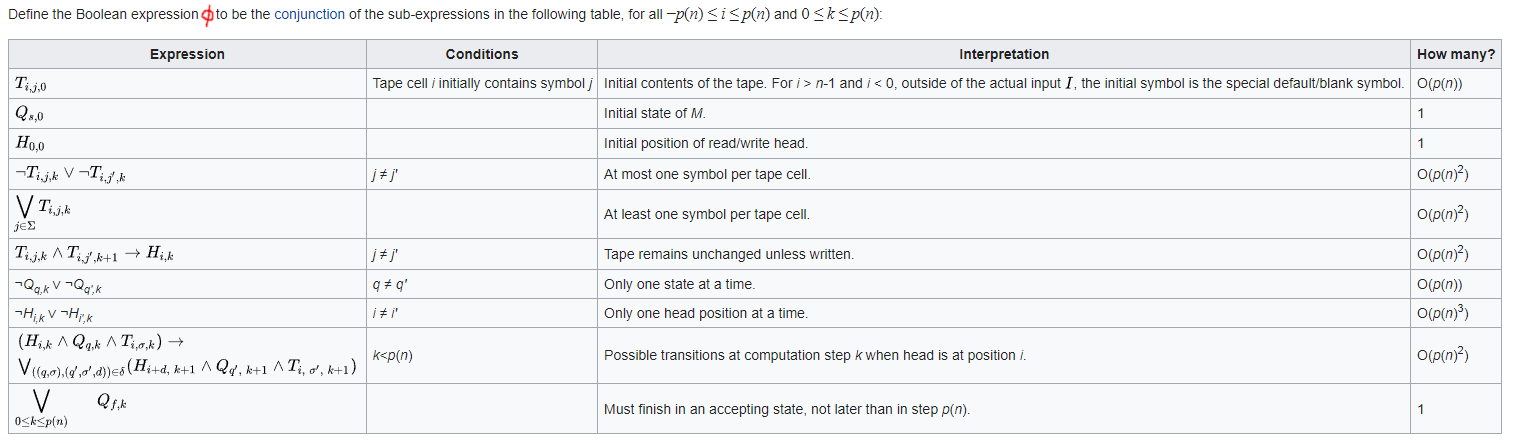
\includegraphics[width=12cm]{img/cook-levin-statement.png}
    
    TL;DR: by choosing an assignment for this statement, we are specifying an \textit{execution path} that the NTM $M$ takes on an input, and vice versa.
\end{figure}


\end{frame}











\end{document}